From the very beginning, I knew I wanted to use Python. I had some slight background knowledge in ML from online courses and most of them were done in Python. Therefore while searching and deciding which library should I use, I have always given a slight edge to the Python options. I have considered (and tested) these:
\begin{itemize}
\item \textbf{NLTK} - probably the best-known Python module for NLP. It provides easy-to-use interfaces for more than 50 corpora and lexical resources. It also offers a rich palette of processing libraries for classification, tokenization, stemming, tagging, parsing, and semantic reasoning.
\item \textbf{Textblob: Simplified Text Processing} - as a name says, Textblob provides easy processing and is actually built on top of NLTK. It provides a simple API for diving into common natural language processing tasks such as part-of-speech tagging, noun phrase extraction, sentiment analysis (Naive Bayes, Decision Tree), classification, translation and more.
\item \textbf{Scikit-learn} - Python module for general ML, data mining and data analysis. It is built on NumPy, SciPy and Matplotlib modules.
\end{itemize}

Also, sentiment analysis is just one part of the task. To evaluate the data and find pattern, basic data science algorithms will be needed. With data science, R is very often listed as a default choice. Therefore were the results of google trends query shown in Figure  pretty surprising. This definitely helped my decision with sticking to Python.

\begin{figure}[H]%
    \centering
	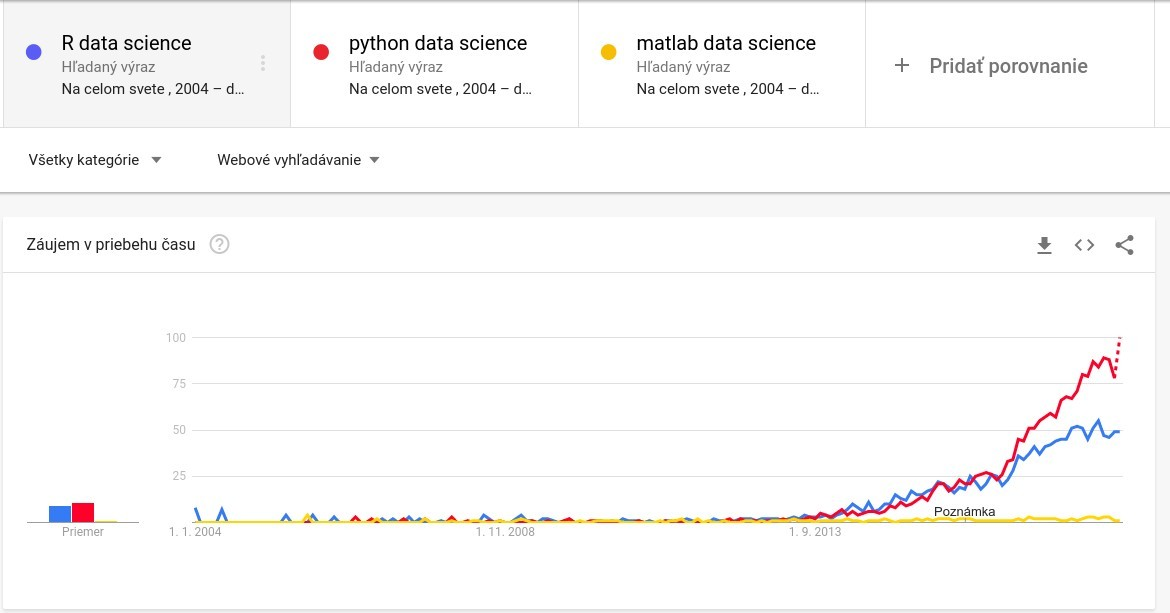
\includegraphics[width=10cm]{PythonMatlabR.jpg}
    \caption{Google trend of searches regarding data science with various programming languages}%
    \label{fig:PythonMatlabR}%
\end{figure}
